\documentclass{article}
\usepackage{amsmath}
\usepackage{color,pxfonts,fix-cm}
\usepackage{latexsym}
\usepackage[mathletters]{ucs}
\DeclareUnicodeCharacter{8226}{$\bullet$}
\usepackage[T1]{fontenc}
\usepackage[utf8x]{inputenc}
\usepackage{pict2e}
\usepackage{wasysym}
\usepackage[english]{babel}
\usepackage{tikz}
\pagestyle{empty}
\usepackage[margin=0in,paperwidth=720pt,paperheight=540pt]{geometry}
\begin{document}
\definecolor{color_29791}{rgb}{0,0,0}
\definecolor{color_232414}{rgb}{0.8,0.8,1}
\definecolor{color_167818}{rgb}{0.545098,0.545098,0.545098}
\definecolor{color_165832}{rgb}{0.537255,0.537255,0.537255}
\definecolor{color_283006}{rgb}{1,1,1}
\begin{tikzpicture}[overlay]\path(0pt,0pt);\end{tikzpicture}
\begin{picture}(-5,0)(2.5,0)
\put(-15,-530){
\includegraphics[width=720pt,height=540pt]{latexImage_432c55c52c2b004ff7b76272af817a3a.png}}
\put(48.45001,-192.1391){\fontsize{28}{1}\usefont{T1}{ptm}{m}{n}\selectfont\color{color_29791}British }
\put(132.478,-192.1391){\fontsize{28}{1}\usefont{T1}{ptm}{m}{n}\selectfont\color{color_29791}Antarctic Survey}
\put(48.45001,-259.3391){\fontsize{28}{1}\usefont{T1}{ptm}{m}{n}\selectfont\color{color_29791}HPC Induction 2021}
\end{picture}
\newpage
\begin{tikzpicture}[overlay]\path(0pt,0pt);\end{tikzpicture}
\begin{picture}(-5,0)(2.5,0)
\put(-15,-530){
\includegraphics[width=720pt,height=540pt]{latexImage_0576cd716feb43c0bdb900476e5c8735.png}}
\put(48.45001,-60.06732){\fontsize{22}{1}\usefont{T1}{ptm}{b}{n}\selectfont\color{color_29791}T}
\put(60.26402,-60.06732){\fontsize{22}{1}\usefont{T1}{ptm}{b}{n}\selectfont\color{color_29791}opics Covered}
\put(48.2,-119.9226){\fontsize{20.5}{1}\usefont{T1}{ptm}{m}{n}\selectfont\color{color_29791}•}
\put(62.2,-119.9226){\fontsize{20}{1}\usefont{T1}{ptm}{m}{n}\selectfont\color{color_29791}Hardware}
\put(48.2,-159.9226){\fontsize{20.5}{1}\usefont{T1}{ptm}{m}{n}\selectfont\color{color_29791}•}
\put(62.2,-159.9226){\fontsize{20}{1}\usefont{T1}{ptm}{m}{n}\selectfont\color{color_29791}Storage}
\put(48.2,-199.9226){\fontsize{20.5}{1}\usefont{T1}{ptm}{m}{n}\selectfont\color{color_29791}•}
\put(62.2,-199.9226){\fontsize{20}{1}\usefont{T1}{ptm}{m}{n}\selectfont\color{color_29791}Access}
\put(48.2,-239.9226){\fontsize{20.5}{1}\usefont{T1}{ptm}{m}{n}\selectfont\color{color_29791}•}
\put(62.2,-239.9226){\fontsize{20}{1}\usefont{T1}{ptm}{m}{n}\selectfont\color{color_29791}Data }
\put(109.64,-239.9226){\fontsize{20}{1}\usefont{T1}{ptm}{m}{n}\selectfont\color{color_29791}T}
\put(121.12,-239.9226){\fontsize{20}{1}\usefont{T1}{ptm}{m}{n}\selectfont\color{color_29791}ransfer}
\put(48.2,-279.9226){\fontsize{20.5}{1}\usefont{T1}{ptm}{m}{n}\selectfont\color{color_29791}•}
\put(62.2,-279.9226){\fontsize{20}{1}\usefont{T1}{ptm}{m}{n}\selectfont\color{color_29791}User Environment}
\put(48.2,-319.9226){\fontsize{20.5}{1}\usefont{T1}{ptm}{m}{n}\selectfont\color{color_29791}•}
\put(62.2,-319.9226){\fontsize{20}{1}\usefont{T1}{ptm}{m}{n}\selectfont\color{color_29791}Software}
\put(349.7,-120.0475){\fontsize{20.5}{1}\usefont{T1}{ptm}{m}{n}\selectfont\color{color_29791}•}
\put(363.7,-120.0475){\fontsize{20}{1}\usefont{T1}{ptm}{m}{n}\selectfont\color{color_29791}Containers}
\put(349.7,-160.0475){\fontsize{20.5}{1}\usefont{T1}{ptm}{m}{n}\selectfont\color{color_29791}•}
\put(363.7,-160.0475){\fontsize{20}{1}\usefont{T1}{ptm}{m}{n}\selectfont\color{color_29791}SLURM}
\put(349.7,-200.0475){\fontsize{20.5}{1}\usefont{T1}{ptm}{m}{n}\selectfont\color{color_29791}•}
\put(363.7,-200.0475){\fontsize{20}{1}\usefont{T1}{ptm}{m}{n}\selectfont\color{color_29791}Model Ensembler}
\put(349.7,-240.0475){\fontsize{20.5}{1}\usefont{T1}{ptm}{m}{n}\selectfont\color{color_29791}•}
\put(363.7,-240.0475){\fontsize{20}{1}\usefont{T1}{ptm}{m}{n}\selectfont\color{color_29791}Best Practice}
\put(349.7,-280.0475){\fontsize{20.5}{1}\usefont{T1}{ptm}{m}{n}\selectfont\color{color_29791}•}
\put(363.7,-280.0475){\fontsize{20}{1}\usefont{T1}{ptm}{m}{n}\selectfont\color{color_29791}HELP!}
\end{picture}
\newpage
\begin{tikzpicture}[overlay]\path(0pt,0pt);\end{tikzpicture}
\begin{picture}(-5,0)(2.5,0)
\put(-15,-530){
\includegraphics[width=720pt,height=540pt]{latexImage_c150d6a5d31e56fa54dc2f27c6d29c24.png}}
\put(48.45001,-60.06732){\fontsize{22}{1}\usefont{T1}{ptm}{b}{n}\selectfont\color{color_29791}Hardware}
\put(48.20001,-116.0331){\fontsize{16.5}{1}\usefont{T1}{ptm}{m}{n}\selectfont\color{color_29791}•}
\put(62.20001,-116.0331){\fontsize{16}{1}\usefont{T1}{ptm}{m}{n}\selectfont\color{color_29791}Gateway or Bastion hosts (}
\put(254.45,-116.0331){\fontsize{12}{1}\usefont{T1}{ptm}{m}{n}\selectfont\color{color_29791}bslcenb \& bslcenc)}
\put(75.70001,-145.3436){\fontsize{12.5}{1}\usefont{T1}{ptm}{m}{n}\selectfont\color{color_29791}•}
\put(98.20001,-145.3436){\fontsize{12}{1}\usefont{T1}{ptm}{m}{n}\selectfont\color{color_29791}Only use for access to BAS or transferring files, don’t use for running programs }
\put(48.20001,-178.6331){\fontsize{16.5}{1}\usefont{T1}{ptm}{m}{n}\selectfont\color{color_29791}•}
\put(62.20001,-178.6331){\fontsize{16}{1}\usefont{T1}{ptm}{m}{n}\selectfont\color{color_29791}Headnodes}
\put(75.70001,-207.9436){\fontsize{12.5}{1}\usefont{T1}{ptm}{m}{n}\selectfont\color{color_29791}•}
\put(98.20001,-207.9436){\fontsize{12}{1}\usefont{T1}{ptm}{m}{n}\selectfont\color{color_29791}No access, manages job queues and storage (/data/hpcdata)}
\put(48.20001,-241.2331){\fontsize{16.5}{1}\usefont{T1}{ptm}{m}{n}\selectfont\color{color_29791}•}
\put(62.20001,-241.2331){\fontsize{16}{1}\usefont{T1}{ptm}{m}{n}\selectfont\color{color_29791}General Use W}
\put(171.272,-241.2331){\fontsize{16}{1}\usefont{T1}{ptm}{m}{n}\selectfont\color{color_29791}orkstations \& Private W}
\put(337.256,-241.2331){\fontsize{16}{1}\usefont{T1}{ptm}{m}{n}\selectfont\color{color_29791}orkstations}
\put(48.20001,-275.4331){\fontsize{16.5}{1}\usefont{T1}{ptm}{m}{n}\selectfont\color{color_29791}•}
\put(62.20001,-275.4331){\fontsize{16}{1}\usefont{T1}{ptm}{m}{n}\selectfont\color{color_29791}Nodes}
\put(48.20001,-309.6331){\fontsize{16.5}{1}\usefont{T1}{ptm}{m}{n}\selectfont\color{color_29791}•}
\put(62.20001,-309.6331){\fontsize{16}{1}\usefont{T1}{ptm}{m}{n}\selectfont\color{color_29791}GPU Nodes}
\put(84.20001,-338.9435){\fontsize{12.5}{1}\usefont{T1}{ptm}{m}{n}\selectfont\color{color_29791}•}
\put(98.20001,-338.9435){\fontsize{12}{1}\usefont{T1}{ptm}{m}{n}\selectfont\color{color_29791}Currently only available for use BAS }
\put(292.948,-338.9435){\fontsize{12}{1}\usefont{T1}{ptm}{m}{n}\selectfont\color{color_29791}AI Lab members}
\put(48.20001,-372.2331){\fontsize{16.5}{1}\usefont{T1}{ptm}{m}{n}\selectfont\color{color_29791}•}
\put(62.20001,-372.2331){\fontsize{16}{1}\usefont{T1}{ptm}{m}{n}\selectfont\color{color_29791}Development W}
\put(175.72,-372.2331){\fontsize{16}{1}\usefont{T1}{ptm}{m}{n}\selectfont\color{color_29791}orkstation and Development Node}
\put(84.20001,-401.5435){\fontsize{12.5}{1}\usefont{T1}{ptm}{m}{n}\selectfont\color{color_29791}•}
\put(98.20001,-401.5435){\fontsize{12}{1}\usefont{T1}{ptm}{m}{n}\selectfont\color{color_29791}No access, used for testing by IT}
\end{picture}
\newpage
\begin{tikzpicture}[overlay]\path(0pt,0pt);\end{tikzpicture}
\begin{picture}(-5,0)(2.5,0)
\put(-15,-530){
\includegraphics[width=720pt,height=540pt]{latexImage_0576cd716feb43c0bdb900476e5c8735.png}}
\put(48.45001,-60.06732){\fontsize{22}{1}\usefont{T1}{ptm}{b}{n}\selectfont\color{color_29791}Access}
\put(48.20001,-116.0331){\fontsize{16}{1}\usefont{T1}{ptm}{m}{n}\selectfont\color{color_29791}Authentication}
\put(84.20001,-145.3436){\fontsize{12.5}{1}\usefont{T1}{ptm}{m}{n}\selectfont\color{color_29791}•}
\put(98.20001,-145.3436){\fontsize{12}{1}\usefont{T1}{ptm}{m}{n}\selectfont\color{color_29791}Three passwords – UNIX (NIS), LDAP}
\put(301.372,-145.3436){\fontsize{12}{1}\usefont{T1}{ptm}{m}{n}\selectfont\color{color_29791} and Samba, }
\put(84.20001,-173.7436){\fontsize{12.5}{1}\usefont{T1}{ptm}{m}{n}\selectfont\color{color_29791}•}
\put(98.20001,-173.7436){\fontsize{12}{1}\usefont{T1}{ptm}{m}{n}\selectfont\color{color_29791}UNIX for bslcenb / bslcenc and LDAP}
\put(297.4,-173.7436){\fontsize{12}{1}\usefont{T1}{ptm}{m}{n}\selectfont\color{color_29791} for HPC workstations}
\put(84.20001,-202.1436){\fontsize{12.5}{1}\usefont{T1}{ptm}{m}{n}\selectfont\color{color_29791}•}
\put(98.20001,-202.1436){\fontsize{12}{1}\usefont{T1}{ptm}{m}{n}\selectfont\color{color_29791}T}
\put(105.088,-202.1436){\fontsize{12}{1}\usefont{T1}{ptm}{m}{n}\selectfont\color{color_29791}ry to keep all these password synchronised}
\put(84.20001,-230.5436){\fontsize{12.5}{1}\usefont{T1}{ptm}{m}{n}\selectfont\color{color_29791}•}
\put(98.20001,-230.5436){\fontsize{12}{1}\usefont{T1}{ptm}{m}{n}\selectfont\color{color_29791}W}
\put(109.312,-230.5436){\fontsize{12}{1}\usefont{T1}{ptm}{m}{n}\selectfont\color{color_29791}e are working to simplify the situation}
\put(48.20001,-263.8331){\fontsize{16}{1}\usefont{T1}{ptm}{m}{n}\selectfont\color{color_29791}SSH}
\put(84.20001,-293.1436){\fontsize{12.5}{1}\usefont{T1}{ptm}{m}{n}\selectfont\color{color_29791}•}
\put(98.20001,-293.1436){\fontsize{12}{1}\usefont{T1}{ptm}{m}{n}\selectfont\color{color_29791}First connect to gateway hosts: bslcenb.nerc-bas.ac.uk / bslcenc.nerc-bas.ac.uk }
\put(84.20001,-321.5436){\fontsize{12.5}{1}\usefont{T1}{ptm}{m}{n}\selectfont\color{color_29791}•}
\put(98.20001,-321.5436){\fontsize{12}{1}\usefont{T1}{ptm}{m}{n}\selectfont\color{color_29791}Second connect to HPC workstations: bslws01 – bslws12}
\put(84.20001,-349.9436){\fontsize{12.5}{1}\usefont{T1}{ptm}{m}{n}\selectfont\color{color_29791}•}
\put(98.20001,-349.9436){\fontsize{12}{1}\usefont{T1}{ptm}{m}{n}\selectfont\color{color_29791}OpenSSH (available for Linux, Mac \& windows), Putty}
\put(383.416,-349.9436){\fontsize{12}{1}\usefont{T1}{ptm}{m}{n}\selectfont\color{color_29791}, WSL, MobaXterm}
\put(48.20001,-383.2331){\fontsize{16}{1}\usefont{T1}{ptm}{m}{n}\selectfont\color{color_29791}Demonstration}
\end{picture}
\newpage
\begin{tikzpicture}[overlay]\path(0pt,0pt);\end{tikzpicture}
\begin{picture}(-5,0)(2.5,0)
\put(-15,-530){
\includegraphics[width=720pt,height=540pt]{latexImage_ce4d9623382f08f383dd59532cc43efc.png}}
\put(48.45001,-60.06732){\fontsize{22}{1}\usefont{T1}{ptm}{b}{n}\selectfont\color{color_29791}Access (continued)}
\put(48.20001,-116.0331){\fontsize{16}{1}\usefont{T1}{ptm}{m}{n}\selectfont\color{color_29791}X2Go}
\put(84.20001,-145.3436){\fontsize{12.5}{1}\usefont{T1}{ptm}{m}{n}\selectfont\color{color_29791}•}
\put(106.7,-145.3436){\fontsize{12}{1}\usefont{T1}{ptm}{m}{n}\selectfont\color{color_29791}Access HPC desktop interface with or without VPN access}
\put(84.20001,-173.7436){\fontsize{12.5}{1}\usefont{T1}{ptm}{m}{n}\selectfont\color{color_29791}•}
\put(106.7,-173.7436){\fontsize{12}{1}\usefont{T1}{ptm}{m}{n}\selectfont\color{color_29791}Disconnecting and reconnecting}
\put(84.20001,-202.1436){\fontsize{12.5}{1}\usefont{T1}{ptm}{m}{n}\selectfont\color{color_29791}•}
\put(106.7,-202.1436){\fontsize{12}{1}\usefont{T1}{ptm}{m}{n}\selectfont\color{color_29791}Copy/paste}
\put(84.20001,-230.5436){\fontsize{12.5}{1}\usefont{T1}{ptm}{m}{n}\selectfont\color{color_29791}•}
\put(106.7,-230.5436){\fontsize{12}{1}\usefont{T1}{ptm}{m}{n}\selectfont\color{color_29791}Sharing files from your laptop or PC}
\put(84.20001,-258.9436){\fontsize{12.5}{1}\usefont{T1}{ptm}{m}{n}\selectfont\color{color_29791}•}
\put(106.7,-258.9436){\fontsize{12}{1}\usefont{T1}{ptm}{m}{n}\selectfont\color{color_29791}More information: }
\put(203.2,-258.9436){\fontsize{12}{1}\usefont{T1}{ptm}{m}{n}\selectfont\color{color_232414}http://ictdocs/wiki/index.php/HPC:X2GO}
\end{picture}
\begin{tikzpicture}[overlay]
\path(0pt,0pt);
\filldraw[color_232414][even odd rule]
(203.2pt, -260.1436pt) -- (414.325pt, -260.1436pt)
;
\end{tikzpicture}
\begin{picture}(-5,0)(2.5,0)
\put(84.20001,-287.3436){\fontsize{12.5}{1}\usefont{T1}{ptm}{m}{n}\selectfont\color{color_29791}•}
\put(106.7,-287.3436){\fontsize{12}{1}\usefont{T1}{ptm}{m}{n}\selectfont\color{color_29791}Demonstration}
\put(48.20001,-320.6331){\fontsize{16}{1}\usefont{T1}{ptm}{m}{n}\selectfont\color{color_29791}Other Options}
\put(84.20001,-349.9436){\fontsize{12.5}{1}\usefont{T1}{ptm}{m}{n}\selectfont\color{color_29791}•}
\put(106.7,-349.9436){\fontsize{12}{1}\usefont{T1}{ptm}{m}{n}\selectfont\color{color_29791}Exceed / XMing}
\put(84.20001,-378.3436){\fontsize{12.5}{1}\usefont{T1}{ptm}{m}{n}\selectfont\color{color_29791}•}
\put(106.7,-378.3436){\fontsize{12}{1}\usefont{T1}{ptm}{m}{n}\selectfont\color{color_29791}MobaXterm}
\put(84.20001,-406.7436){\fontsize{12.5}{1}\usefont{T1}{ptm}{m}{n}\selectfont\color{color_29791}•}
\put(106.7,-406.7436){\fontsize{12}{1}\usefont{T1}{ptm}{m}{n}\selectfont\color{color_29791}Demonstration}
\end{picture}
\newpage
\begin{tikzpicture}[overlay]\path(0pt,0pt);\end{tikzpicture}
\begin{picture}(-5,0)(2.5,0)
\put(-15,-530){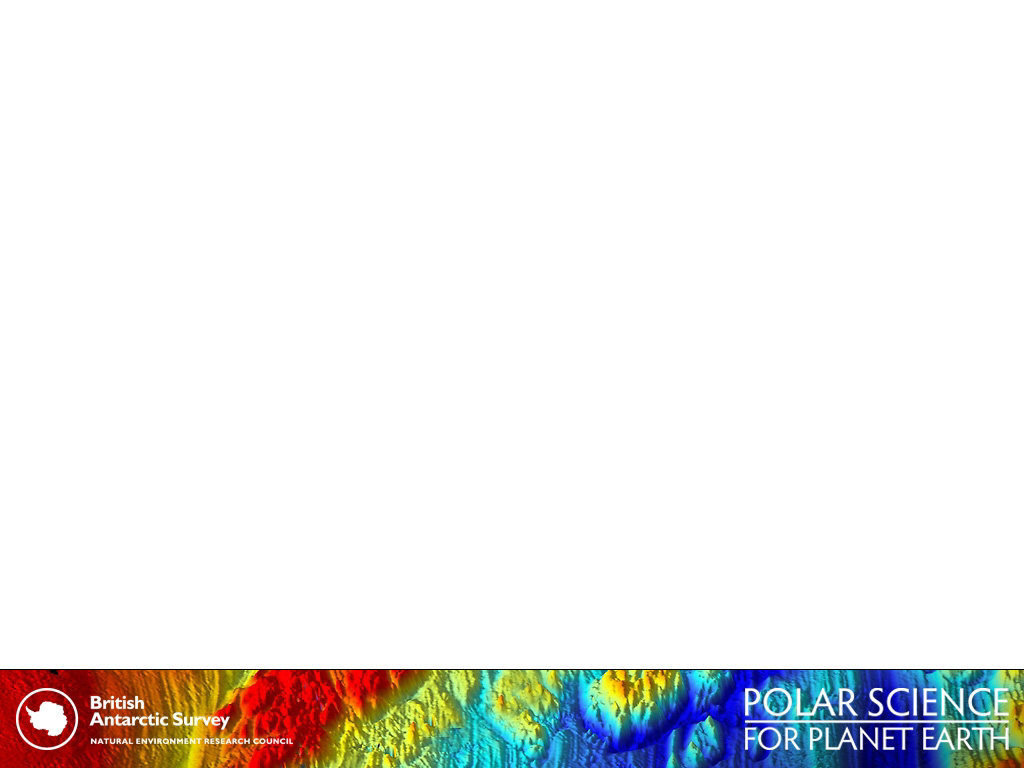
\includegraphics[width=720pt,height=540pt]{latexImage_0bbbcdc264c8ba747f2e5d9a88383de2.png}}
\put(48.45001,-60.06732){\fontsize{22}{1}\usefont{T1}{ptm}{b}{n}\selectfont\color{color_29791}Storage}
\put(48.20001,-116.0331){\fontsize{16}{1}\usefont{T1}{ptm}{m}{n}\selectfont\color{color_29791}User }
\put(85.54401,-116.0331){\fontsize{16}{1}\usefont{T1}{ptm}{m}{n}\selectfont\color{color_29791}Area - /users/username}
\put(84.20001,-145.3436){\fontsize{12.5}{1}\usefont{T1}{ptm}{m}{n}\selectfont\color{color_29791}•}
\put(98.20001,-145.3436){\fontsize{12}{1}\usefont{T1}{ptm}{m}{n}\selectfont\color{color_29791}Small, not intended for sharing data}
\put(84.20001,-173.7436){\fontsize{12.5}{1}\usefont{T1}{ptm}{m}{n}\selectfont\color{color_29791}•}
\put(98.20001,-173.7436){\fontsize{12}{1}\usefont{T1}{ptm}{m}{n}\selectfont\color{color_29791}Space restricted via quotas}
\put(48.20001,-207.0331){\fontsize{16}{1}\usefont{T1}{ptm}{m}{n}\selectfont\color{color_29791}SAN V}
\put(95.33601,-207.0331){\fontsize{16}{1}\usefont{T1}{ptm}{m}{n}\selectfont\color{color_29791}olumes}
\put(84.20001,-236.3436){\fontsize{12.5}{1}\usefont{T1}{ptm}{m}{n}\selectfont\color{color_29791}•}
\put(98.20001,-236.3436){\fontsize{12}{1}\usefont{T1}{ptm}{m}{n}\selectfont\color{color_29791}Setup for projects and departments, eg: : /data/cruise, /data/vlf}
\put(84.20001,-264.7436){\fontsize{12.5}{1}\usefont{T1}{ptm}{m}{n}\selectfont\color{color_29791}•}
\put(98.20001,-264.7436){\fontsize{12}{1}\usefont{T1}{ptm}{m}{n}\selectfont\color{color_29791}Accessible from workstations, bslcenb, bslcenc}
\put(84.20001,-293.1436){\fontsize{12.5}{1}\usefont{T1}{ptm}{m}{n}\selectfont\color{color_29791}•}
\put(98.20001,-293.1436){\fontsize{12}{1}\usefont{T1}{ptm}{m}{n}\selectfont\color{color_29791}V}
\put(105.544,-293.1436){\fontsize{12}{1}\usefont{T1}{ptm}{m}{n}\selectfont\color{color_29791}olume should be managed and curated by a data manager}
\put(84.20001,-321.5436){\fontsize{12.5}{1}\usefont{T1}{ptm}{m}{n}\selectfont\color{color_29791}•}
\put(98.20001,-321.5436){\fontsize{12}{1}\usefont{T1}{ptm}{m}{n}\selectfont\color{color_29791}Space is not controlled by quota's}
\put(84.20001,-349.9436){\fontsize{12.5}{1}\usefont{T1}{ptm}{m}{n}\selectfont\color{color_29791}•}
\put(98.20001,-349.9436){\fontsize{12}{1}\usefont{T1}{ptm}{m}{n}\selectfont\color{color_29791}Adding additional space depends availability of physical disk space}
\put(84.20001,-378.3436){\fontsize{12.5}{1}\usefont{T1}{ptm}{m}{n}\selectfont\color{color_29791}•}
\put(98.20001,-378.3436){\fontsize{12}{1}\usefont{T1}{ptm}{m}{n}\selectfont\color{color_29791}Contact data manager first if you think you require additional storage}
\end{picture}
\newpage
\begin{tikzpicture}[overlay]\path(0pt,0pt);\end{tikzpicture}
\begin{picture}(-5,0)(2.5,0)
\put(-15,-530){
\includegraphics[width=720pt,height=540pt]{latexImage_74554d3b0f5b45b9b07769003a1a7e32.png}}
\put(48.45001,-60.06732){\fontsize{22}{1}\usefont{T1}{ptm}{b}{n}\selectfont\color{color_29791}Storage (continued)}
\put(48.20001,-116.0331){\fontsize{16}{1}\usefont{T1}{ptm}{m}{n}\selectfont\color{color_29791}HPC Storage - /data/hpcdata/ (users, data) \& /data/hpcflash}
\put(84.20001,-145.3436){\fontsize{12.5}{1}\usefont{T1}{ptm}{m}{n}\selectfont\color{color_29791}•}
\put(98.20001,-145.3436){\fontsize{12}{1}\usefont{T1}{ptm}{m}{n}\selectfont\color{color_29791}Accessible from nodes and workstations, bslcenb, bslcenc.}
\put(84.20001,-173.7436){\fontsize{12.5}{1}\usefont{T1}{ptm}{m}{n}\selectfont\color{color_29791}•}
\put(98.20001,-173.7436){\fontsize{12}{1}\usefont{T1}{ptm}{m}{n}\selectfont\color{color_29791}Usage limited via quotas}
\put(48.20001,-207.0331){\fontsize{16}{1}\usefont{T1}{ptm}{m}{n}\selectfont\color{color_29791}Quotas}
\put(84.20001,-236.3436){\fontsize{12.5}{1}\usefont{T1}{ptm}{m}{n}\selectfont\color{color_29791}•}
\put(97.70001,-236.3436){\fontsize{12}{1}\usefont{T1}{ptm}{m}{n}\selectfont\color{color_29791}On HPC you can check your quotas using: myquota}
\put(84.20001,-264.7436){\fontsize{12.5}{1}\usefont{T1}{ptm}{m}{n}\selectfont\color{color_29791}•}
\put(97.70001,-264.7436){\fontsize{12}{1}\usefont{T1}{ptm}{m}{n}\selectfont\color{color_29791}Need more space - contact the service desk}
\put(48.20001,-298.0331){\fontsize{16}{1}\usefont{T1}{ptm}{m}{n}\selectfont\color{color_29791}Backups }
\put(84.20001,-327.3436){\fontsize{12.5}{1}\usefont{T1}{ptm}{m}{n}\selectfont\color{color_29791}•}
\put(98.20001,-327.3436){\fontsize{12}{1}\usefont{T1}{ptm}{m}{n}\selectfont\color{color_29791}Daily at 6pm}
\put(84.20001,-355.7436){\fontsize{12.5}{1}\usefont{T1}{ptm}{m}{n}\selectfont\color{color_29791}•}
\put(98.20001,-355.7436){\fontsize{12}{1}\usefont{T1}{ptm}{m}{n}\selectfont\color{color_29791}All SAN and HPC volumes backed up}
\put(84.20001,-384.1436){\fontsize{12.5}{1}\usefont{T1}{ptm}{m}{n}\selectfont\color{color_29791}•}
\put(98.20001,-384.1436){\fontsize{12}{1}\usefont{T1}{ptm}{m}{n}\selectfont\color{color_29791}Backups are both onsite and of}
\put(263.416,-384.1436){\fontsize{12}{1}\usefont{T1}{ptm}{m}{n}\selectfont\color{color_29791}fsite, via tapes \& disk}
\put(84.20001,-412.5436){\fontsize{12.5}{1}\usefont{T1}{ptm}{m}{n}\selectfont\color{color_29791}•}
\put(98.20001,-412.5436){\fontsize{12}{1}\usefont{T1}{ptm}{m}{n}\selectfont\color{color_29791}If you need a file restored, contact the service desk}
\end{picture}
\newpage
\begin{tikzpicture}[overlay]\path(0pt,0pt);\end{tikzpicture}
\begin{picture}(-5,0)(2.5,0)
\put(-15,-530){
\includegraphics[width=720pt,height=540pt]{latexImage_0c7e336018b624b6d33eacc011f59acd.png}}
\put(48.45001,-60.06732){\fontsize{22}{1}\usefont{T1}{ptm}{b}{n}\selectfont\color{color_29791}Data }
\put(101.426,-60.06732){\fontsize{22}{1}\usefont{T1}{ptm}{b}{n}\selectfont\color{color_29791}Access and T}
\put(242.05,-60.06732){\fontsize{22}{1}\usefont{T1}{ptm}{b}{n}\selectfont\color{color_29791}ransfer}
\put(48.20001,-116.0331){\fontsize{16}{1}\usefont{T1}{ptm}{m}{n}\selectfont\color{color_29791}Samba }
\put(84.20001,-145.3436){\fontsize{12.5}{1}\usefont{T1}{ptm}{m}{n}\selectfont\color{color_29791}•}
\put(98.20001,-145.3436){\fontsize{12}{1}\usefont{T1}{ptm}{m}{n}\selectfont\color{color_29791}Allows clients to connect to UNIX storage as if it were a windows network share.}
\put(84.20001,-173.7436){\fontsize{12.5}{1}\usefont{T1}{ptm}{m}{n}\selectfont\color{color_29791}•}
\put(98.20001,-173.7436){\fontsize{12}{1}\usefont{T1}{ptm}{m}{n}\selectfont\color{color_29791}Allows access to SAN volumes, /users and /data/hpcdata}
\put(84.20001,-202.1436){\fontsize{12.5}{1}\usefont{T1}{ptm}{m}{n}\selectfont\color{color_29791}•}
\put(98.20001,-202.1436){\fontsize{12}{1}\usefont{T1}{ptm}{m}{n}\selectfont\color{color_29791}No access to /data/hpcflash}
\put(48.20001,-235.4331){\fontsize{16}{1}\usefont{T1}{ptm}{m}{n}\selectfont\color{color_29791}FTP}
\put(84.20001,-264.7436){\fontsize{12.5}{1}\usefont{T1}{ptm}{m}{n}\selectfont\color{color_29791}•}
\put(98.20001,-264.7436){\fontsize{12}{1}\usefont{T1}{ptm}{m}{n}\selectfont\color{color_29791}Allows non-BAS users to retrieve files from the FTP}
\put(371.404,-264.7436){\fontsize{12}{1}\usefont{T1}{ptm}{m}{n}\selectfont\color{color_29791} area }
\put(401.95,-264.7436){\fontsize{12}{1}\usefont{T1}{ptm}{m}{n}\selectfont\color{color_232414}ftp://ftp.bas.ac.uk/}
\end{picture}
\begin{tikzpicture}[overlay]
\path(0pt,0pt);
\filldraw[color_232414][even odd rule]
(401.95pt, -265.9435pt) -- (496.825pt, -265.9435pt)
;
\end{tikzpicture}
\begin{picture}(-5,0)(2.5,0)
\put(496.825,-264.7436){\fontsize{12}{1}\usefont{T1}{ptm}{m}{n}\selectfont\color{color_29791} }
\put(84.20001,-293.1436){\fontsize{12.5}{1}\usefont{T1}{ptm}{m}{n}\selectfont\color{color_29791}•}
\put(98.20001,-293.1436){\fontsize{12}{1}\usefont{T1}{ptm}{m}{n}\selectfont\color{color_29791}Users within BAS can gain access to this area and deposit files}
\put(84.20001,-321.5436){\fontsize{12.5}{1}\usefont{T1}{ptm}{m}{n}\selectfont\color{color_29791}•}
\put(98.20001,-321.5436){\fontsize{12}{1}\usefont{T1}{ptm}{m}{n}\selectfont\color{color_29791}Please contact the IT}
\put(210.712,-321.5436){\fontsize{12}{1}\usefont{T1}{ptm}{m}{n}\selectfont\color{color_29791} ServiceDesk to have a directory setup ie. /data/ftp/username }
\put(48.20001,-354.8331){\fontsize{16}{1}\usefont{T1}{ptm}{m}{n}\selectfont\color{color_29791}W}
\put(63.01601,-354.8331){\fontsize{16}{1}\usefont{T1}{ptm}{m}{n}\selectfont\color{color_29791}riteable FTP}
\put(149.864,-354.8331){\fontsize{16}{1}\usefont{T1}{ptm}{m}{n}\selectfont\color{color_29791} }
\put(153.432,-354.8331){\fontsize{16}{1}\usefont{T1}{ptm}{m}{n}\selectfont\color{color_29791}Area}
\put(84.20001,-384.1436){\fontsize{12.5}{1}\usefont{T1}{ptm}{m}{n}\selectfont\color{color_29791}•}
\put(98.20001,-384.1436){\fontsize{12}{1}\usefont{T1}{ptm}{m}{n}\selectfont\color{color_29791}Possible for non-BAS users to upload files as well, please contact the IT}
\put(480.16,-384.1436){\fontsize{12}{1}\usefont{T1}{ptm}{m}{n}\selectfont\color{color_29791} ServiceDesk for details}
\end{picture}
\newpage
\begin{tikzpicture}[overlay]\path(0pt,0pt);\end{tikzpicture}
\begin{picture}(-5,0)(2.5,0)
\put(-15,-530){
\includegraphics[width=720pt,height=540pt]{latexImage_8e9c8e6734598745b849b301599f41ac.png}}
\put(48.45001,-60.06732){\fontsize{22}{1}\usefont{T1}{ptm}{b}{n}\selectfont\color{color_29791}Data }
\put(101.426,-60.06732){\fontsize{22}{1}\usefont{T1}{ptm}{b}{n}\selectfont\color{color_29791}Access and T}
\put(242.05,-60.06732){\fontsize{22}{1}\usefont{T1}{ptm}{b}{n}\selectfont\color{color_29791}ransfer (continued)}
\put(48.20001,-116.0331){\fontsize{16.5}{1}\usefont{T1}{ptm}{m}{n}\selectfont\color{color_29791}•}
\put(62.20001,-116.0331){\fontsize{16}{1}\usefont{T1}{ptm}{m}{n}\selectfont\color{color_29791}rsync}
\put(84.20001,-145.3436){\fontsize{12.5}{1}\usefont{T1}{ptm}{m}{n}\selectfont\color{color_29791}•}
\put(106.7,-145.3436){\fontsize{12}{1}\usefont{T1}{ptm}{m}{n}\selectfont\color{color_29791}Perfect tool for transferring file locally and securely over the internet}
\put(84.20001,-173.7436){\fontsize{12.5}{1}\usefont{T1}{ptm}{m}{n}\selectfont\color{color_29791}•}
\put(106.7,-173.7436){\fontsize{12}{1}\usefont{T1}{ptm}{m}{n}\selectfont\color{color_29791}Options to resume, reconnect, compression, limit transferred rates.}
\put(48.20001,-207.0331){\fontsize{16.5}{1}\usefont{T1}{ptm}{m}{n}\selectfont\color{color_29791}•}
\put(62.20001,-207.0331){\fontsize{16}{1}\usefont{T1}{ptm}{m}{n}\selectfont\color{color_29791}scp}
\put(48.20001,-241.2331){\fontsize{16.5}{1}\usefont{T1}{ptm}{m}{n}\selectfont\color{color_29791}•}
\put(62.20001,-241.2331){\fontsize{16}{1}\usefont{T1}{ptm}{m}{n}\selectfont\color{color_29791}sshfs}
\end{picture}
\newpage
\begin{tikzpicture}[overlay]\path(0pt,0pt);\end{tikzpicture}
\begin{picture}(-5,0)(2.5,0)
\put(-15,-530){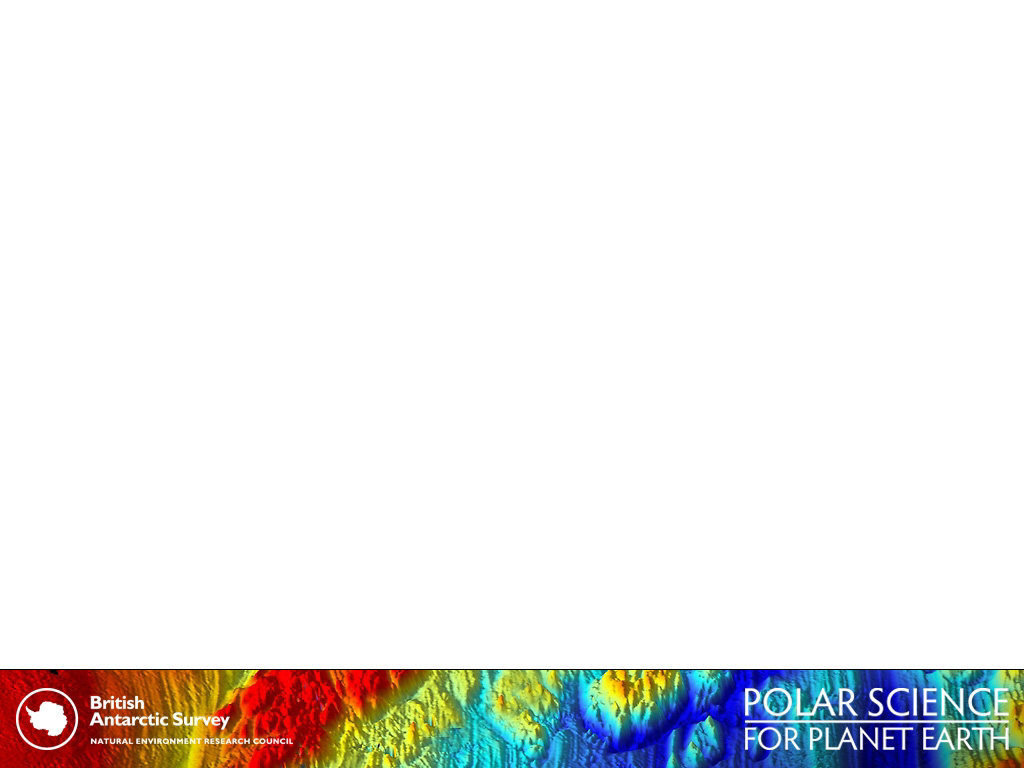
\includegraphics[width=720pt,height=540pt]{latexImage_0bbbcdc264c8ba747f2e5d9a88383de2.png}}
\put(48.45001,-60.06732){\fontsize{22}{1}\usefont{T1}{ptm}{b}{n}\selectfont\color{color_29791}User Environment}
\put(48.20001,-116.0331){\fontsize{16.5}{1}\usefont{T1}{ptm}{m}{n}\selectfont\color{color_29791}•}
\put(62.20001,-116.0331){\fontsize{16}{1}\usefont{T1}{ptm}{m}{n}\selectfont\color{color_29791}Shell }
\put(84.20001,-145.3436){\fontsize{12.5}{1}\usefont{T1}{ptm}{m}{n}\selectfont\color{color_29791}•}
\put(98.20001,-145.3436){\fontsize{12}{1}\usefont{T1}{ptm}{m}{n}\selectfont\color{color_29791}Our default shell is tcsh}
\put(84.20001,-173.7436){\fontsize{12.5}{1}\usefont{T1}{ptm}{m}{n}\selectfont\color{color_29791}•}
\put(98.20001,-173.7436){\fontsize{12}{1}\usefont{T1}{ptm}{m}{n}\selectfont\color{color_29791}If you prefer something dif}
\put(236.716,-173.7436){\fontsize{12}{1}\usefont{T1}{ptm}{m}{n}\selectfont\color{color_29791}ferent such as bash, contact the service desk}
\put(48.20001,-207.0331){\fontsize{16.5}{1}\usefont{T1}{ptm}{m}{n}\selectfont\color{color_29791}•}
\put(62.20001,-207.0331){\fontsize{16}{1}\usefont{T1}{ptm}{m}{n}\selectfont\color{color_29791}SSH keys}
\put(84.20001,-236.3436){\fontsize{12.5}{1}\usefont{T1}{ptm}{m}{n}\selectfont\color{color_29791}•}
\put(98.20001,-236.3436){\fontsize{12}{1}\usefont{T1}{ptm}{m}{n}\selectfont\color{color_29791}Connect to BAS systems without typing passwords}
\put(84.20001,-264.7436){\fontsize{12.5}{1}\usefont{T1}{ptm}{m}{n}\selectfont\color{color_29791}•}
\put(98.20001,-264.7436){\fontsize{12}{1}\usefont{T1}{ptm}{m}{n}\selectfont\color{color_29791}ssh-keygen – }
\put(172.24,-264.7436){\fontsize{12}{1}\usefont{T1}{ptm}{m}{n}\selectfont\color{color_29791}Always create with a passphrase}
\put(84.20001,-293.1436){\fontsize{12.5}{1}\usefont{T1}{ptm}{m}{n}\selectfont\color{color_29791}•}
\put(98.20001,-293.1436){\fontsize{12}{1}\usefont{T1}{ptm}{m}{n}\selectfont\color{color_29791}ssh-agent}
\put(84.20001,-321.5436){\fontsize{12.5}{1}\usefont{T1}{ptm}{m}{n}\selectfont\color{color_29791}•}
\put(98.20001,-321.5436){\fontsize{12}{1}\usefont{T1}{ptm}{m}{n}\selectfont\color{color_29791}./ssh/config}
\put(84.20001,-349.9436){\fontsize{12.5}{1}\usefont{T1}{ptm}{m}{n}\selectfont\color{color_29791}•}
\put(98.20001,-349.9436){\fontsize{12}{1}\usefont{T1}{ptm}{m}{n}\selectfont\color{color_29791}More information: }
\put(194.7,-349.9436){\fontsize{12}{1}\usefont{T1}{ptm}{m}{n}\selectfont\color{color_232414}http://ictdocs/wiki/index.php/SSH\_Keys}
\end{picture}
\begin{tikzpicture}[overlay]
\path(0pt,0pt);
\filldraw[color_232414][even odd rule]
(194.7pt, -351.1436pt) -- (401.7pt, -351.1436pt)
;
\end{tikzpicture}
\begin{picture}(-5,0)(2.5,0)
\put(84.20001,-378.3436){\fontsize{12.5}{1}\usefont{T1}{ptm}{m}{n}\selectfont\color{color_29791}•}
\put(98.20001,-378.3436){\fontsize{12}{1}\usefont{T1}{ptm}{m}{n}\selectfont\color{color_29791}Demonstration}
\end{picture}
\newpage
\begin{tikzpicture}[overlay]\path(0pt,0pt);\end{tikzpicture}
\begin{picture}(-5,0)(2.5,0)
\put(-15,-530){
\includegraphics[width=720pt,height=540pt]{latexImage_c150d6a5d31e56fa54dc2f27c6d29c24.png}}
\put(48.45001,-60.06732){\fontsize{22}{1}\usefont{T1}{ptm}{b}{n}\selectfont\color{color_29791}User Environment}
\put(48.20001,-116.0331){\fontsize{16.5}{1}\usefont{T1}{ptm}{m}{n}\selectfont\color{color_29791}•}
\put(62.20001,-116.0331){\fontsize{16}{1}\usefont{T1}{ptm}{m}{n}\selectfont\color{color_29791}tmux}
\put(84.20001,-145.3436){\fontsize{12.5}{1}\usefont{T1}{ptm}{m}{n}\selectfont\color{color_29791}•}
\put(98.20001,-145.3436){\fontsize{12}{1}\usefont{T1}{ptm}{m}{n}\selectfont\color{color_29791}Keeps long running command line sessions running }
\put(84.20001,-173.7436){\fontsize{12.5}{1}\usefont{T1}{ptm}{m}{n}\selectfont\color{color_29791}•}
\put(98.20001,-173.7436){\fontsize{12}{1}\usefont{T1}{ptm}{m}{n}\selectfont\color{color_29791}Allows disconnecting and reconnecting}
\put(84.20001,-202.1436){\fontsize{12.5}{1}\usefont{T1}{ptm}{m}{n}\selectfont\color{color_29791}•}
\put(98.20001,-202.1436){\fontsize{12}{1}\usefont{T1}{ptm}{m}{n}\selectfont\color{color_29791}Multiple command line sessions and console splitting}
\put(84.20001,-230.5436){\fontsize{12.5}{1}\usefont{T1}{ptm}{m}{n}\selectfont\color{color_29791}•}
\put(98.20001,-230.5436){\fontsize{12}{1}\usefont{T1}{ptm}{m}{n}\selectfont\color{color_29791}More information: }
\put(194.7,-230.5436){\fontsize{12}{1}\usefont{T1}{ptm}{m}{n}\selectfont\color{color_232414}http://ictdocs/wiki/index.php/tmux}
\end{picture}
\begin{tikzpicture}[overlay]
\path(0pt,0pt);
\filldraw[color_232414][even odd rule]
(194.7pt, -231.7436pt) -- (369.825pt, -231.7436pt)
;
\end{tikzpicture}
\begin{picture}(-5,0)(2.5,0)
\put(84.20001,-258.9436){\fontsize{12.5}{1}\usefont{T1}{ptm}{m}{n}\selectfont\color{color_29791}•}
\put(98.20001,-258.9436){\fontsize{12}{1}\usefont{T1}{ptm}{m}{n}\selectfont\color{color_29791}Demonstration}
\end{picture}
\newpage
\begin{tikzpicture}[overlay]\path(0pt,0pt);\end{tikzpicture}
\begin{picture}(-5,0)(2.5,0)
\put(-15,-530){
\includegraphics[width=720pt,height=540pt]{latexImage_0576cd716feb43c0bdb900476e5c8735.png}}
\put(48.45001,-60.06732){\fontsize{22}{1}\usefont{T1}{ptm}{b}{n}\selectfont\color{color_29791}Software}
\put(48.20001,-116.0331){\fontsize{16}{1}\usefont{T1}{ptm}{m}{n}\selectfont\color{color_29791}Operating System software}
\put(84.20001,-145.3436){\fontsize{12.5}{1}\usefont{T1}{ptm}{m}{n}\selectfont\color{color_29791}•}
\put(106.7,-145.3436){\fontsize{12}{1}\usefont{T1}{ptm}{m}{n}\selectfont\color{color_29791}T}
\put(113.372,-145.3436){\fontsize{12}{1}\usefont{T1}{ptm}{m}{n}\selectfont\color{color_29791}ypical linux commands and some graphical packages are installed as part of OS.}
\put(84.20001,-173.7436){\fontsize{12.5}{1}\usefont{T1}{ptm}{m}{n}\selectfont\color{color_29791}•}
\put(106.7,-173.7436){\fontsize{12}{1}\usefont{T1}{ptm}{m}{n}\selectfont\color{color_29791}These can be run from the command line and desktop interface}
\put(48.20001,-204.0331){\fontsize{16}{1}\usefont{T1}{ptm}{m}{n}\selectfont\color{color_29791}Modules}
\put(84.20001,-221.3436){\fontsize{12.5}{1}\usefont{T1}{ptm}{m}{n}\selectfont\color{color_29791}•}
\put(106.7,-221.3436){\fontsize{12}{1}\usefont{T1}{ptm}{m}{n}\selectfont\color{color_29791}Do not work on bslcenb or bslcenc}
\put(84.20001,-249.7436){\fontsize{12.5}{1}\usefont{T1}{ptm}{m}{n}\selectfont\color{color_29791}•}
\put(106.7,-249.7436){\fontsize{12}{1}\usefont{T1}{ptm}{m}{n}\selectfont\color{color_29791}There are two module repositories: /packages/modules \& /hpcpackages/modules }
\put(84.20001,-278.1436){\fontsize{12.5}{1}\usefont{T1}{ptm}{m}{n}\selectfont\color{color_29791}•}
\put(106.7,-278.1436){\fontsize{12}{1}\usefont{T1}{ptm}{m}{n}\selectfont\color{color_29791}Prefer /hpcpackages/modules - works with nodes and workstations}
\put(84.20001,-306.5436){\fontsize{12.5}{1}\usefont{T1}{ptm}{m}{n}\selectfont\color{color_29791}•}
\put(106.7,-306.5436){\fontsize{12}{1}\usefont{T1}{ptm}{m}{n}\selectfont\color{color_29791}Modules sometimes include the compiler used in their name eg. hpc/netcdf/intel/4.4.1.1}
\put(84.20001,-334.9436){\fontsize{12.5}{1}\usefont{T1}{ptm}{m}{n}\selectfont\color{color_29791}•}
\put(106.7,-334.9436){\fontsize{12}{1}\usefont{T1}{ptm}{m}{n}\selectfont\color{color_29791}W}
\put(117.812,-334.9436){\fontsize{12}{1}\usefont{T1}{ptm}{m}{n}\selectfont\color{color_29791}orks by adjusting shell variables eg. P}
\put(317.672,-334.9436){\fontsize{12}{1}\usefont{T1}{ptm}{m}{n}\selectfont\color{color_29791}A}
\put(324.788,-334.9436){\fontsize{12}{1}\usefont{T1}{ptm}{m}{n}\selectfont\color{color_29791}TH, LD\_LIBRAR}
\put(412.592,-334.9436){\fontsize{12}{1}\usefont{T1}{ptm}{m}{n}\selectfont\color{color_29791}Y\_P}
\put(434.384,-334.9436){\fontsize{12}{1}\usefont{T1}{ptm}{m}{n}\selectfont\color{color_29791}A}
\put(441.5,-334.9436){\fontsize{12}{1}\usefont{T1}{ptm}{m}{n}\selectfont\color{color_29791}TH}
\put(84.20001,-363.3436){\fontsize{12.5}{1}\usefont{T1}{ptm}{m}{n}\selectfont\color{color_29791}•}
\put(106.7,-363.3436){\fontsize{12}{1}\usefont{T1}{ptm}{m}{n}\selectfont\color{color_29791}Loaded modules only af}
\put(233.888,-363.3436){\fontsize{12}{1}\usefont{T1}{ptm}{m}{n}\selectfont\color{color_29791}fect the terminal your loaded them in}
\end{picture}
\newpage
\begin{tikzpicture}[overlay]\path(0pt,0pt);\end{tikzpicture}
\begin{picture}(-5,0)(2.5,0)
\put(-15,-530){
\includegraphics[width=720pt,height=540pt]{latexImage_74554d3b0f5b45b9b07769003a1a7e32.png}}
\put(48.45001,-60.06732){\fontsize{22}{1}\usefont{T1}{ptm}{b}{n}\selectfont\color{color_29791}Software (continued)}
\put(48.20001,-116.0331){\fontsize{16}{1}\usefont{T1}{ptm}{m}{n}\selectfont\color{color_29791}Modules}
\put(84.20001,-133.3436){\fontsize{12.5}{1}\usefont{T1}{ptm}{m}{n}\selectfont\color{color_29791}•}
\put(106.7,-133.3436){\fontsize{12}{1}\usefont{T1}{ptm}{m}{n}\selectfont\color{color_29791}Useful module commands: }
\put(120.2,-158.894){\fontsize{10}{1}\usefont{T1}{ptm}{m}{n}\selectfont\color{color_29791}module avail                            module display name/version}
\put(120.2,-184.894){\fontsize{10}{1}\usefont{T1}{ptm}{m}{n}\selectfont\color{color_29791}module load name/version                module list }
\put(120.2,-210.894){\fontsize{10}{1}\usefont{T1}{ptm}{m}{n}\selectfont\color{color_29791}module unload name/version              module purge}
\put(84.20001,-239.7436){\fontsize{12.5}{1}\usefont{T1}{ptm}{m}{n}\selectfont\color{color_29791}•}
\put(106.7,-239.7436){\fontsize{12}{1}\usefont{T1}{ptm}{m}{n}\selectfont\color{color_29791}Common mistakes}
\put(129.2,-268.1436){\fontsize{12.5}{1}\usefont{T1}{ptm}{m}{n}\selectfont\color{color_29791}•}
\put(142.7,-268.1436){\fontsize{12}{1}\usefont{T1}{ptm}{m}{n}\selectfont\color{color_29791}Forgetting to use hpc modules on nodes}
\put(129.2,-296.5436){\fontsize{12.5}{1}\usefont{T1}{ptm}{m}{n}\selectfont\color{color_29791}•}
\put(142.7,-296.5436){\fontsize{12}{1}\usefont{T1}{ptm}{m}{n}\selectfont\color{color_29791}Mixing modules created using dif}
\put(317.216,-296.5436){\fontsize{12}{1}\usefont{T1}{ptm}{m}{n}\selectfont\color{color_29791}ferent compilers}
\put(129.2,-324.9436){\fontsize{12.5}{1}\usefont{T1}{ptm}{m}{n}\selectfont\color{color_29791}•}
\put(142.7,-324.9436){\fontsize{12}{1}\usefont{T1}{ptm}{m}{n}\selectfont\color{color_29791}Loading clashing modules}
\put(84.20001,-353.3436){\fontsize{12.5}{1}\usefont{T1}{ptm}{m}{n}\selectfont\color{color_29791}•}
\put(106.7,-353.3436){\fontsize{12}{1}\usefont{T1}{ptm}{m}{n}\selectfont\color{color_29791}More information: }
\put(203.2,-353.3436){\fontsize{12}{1}\usefont{T1}{ptm}{m}{n}\selectfont\color{color_232414}http://ictdocs/wiki/index.php?title=HPC:User\_Guide}
\end{picture}
\begin{tikzpicture}[overlay]
\path(0pt,0pt);
\filldraw[color_232414][even odd rule]
(203.2pt, -354.5436pt) -- (473.575pt, -354.5436pt)
;
\end{tikzpicture}
\begin{picture}(-5,0)(2.5,0)
\put(84.20001,-381.7436){\fontsize{12.5}{1}\usefont{T1}{ptm}{m}{n}\selectfont\color{color_29791}•}
\put(106.7,-381.7436){\fontsize{12}{1}\usefont{T1}{ptm}{m}{n}\selectfont\color{color_29791}Demonstration}
\end{picture}
\newpage
\begin{tikzpicture}[overlay]\path(0pt,0pt);\end{tikzpicture}
\begin{picture}(-5,0)(2.5,0)
\put(-15,-530){
\includegraphics[width=720pt,height=540pt]{latexImage_0c7e336018b624b6d33eacc011f59acd.png}}
\put(48.45001,-60.06732){\fontsize{22}{1}\usefont{T1}{ptm}{b}{n}\selectfont\color{color_29791}Jupyter Notebooks}
\put(48.20001,-116.0331){\fontsize{16.5}{1}\usefont{T1}{ptm}{m}{n}\selectfont\color{color_29791}•}
\put(62.20001,-116.0331){\fontsize{16}{1}\usefont{T1}{ptm}{m}{n}\selectfont\color{color_29791}Jupter notebooks running on workstations:}
\put(362.825,-116.0331){\fontsize{16}{1}\usefont{T1}{ptm}{m}{n}\selectfont\color{color_167818} }
\put(367.325,-116.0331){\fontsize{16}{1}\usefont{T1}{ptm}{m}{n}\selectfont\color{color_232414}http://jupyterhub.nerc-bas.ac.uk}
\end{picture}
\begin{tikzpicture}[overlay]
\path(0pt,0pt);
\filldraw[color_232414][even odd rule]
(367.325pt, -117.6331pt) -- (591.7pt, -117.6331pt)
;
\end{tikzpicture}
\begin{picture}(-5,0)(2.5,0)
\put(48.20001,-150.2331){\fontsize{16.5}{1}\usefont{T1}{ptm}{m}{n}\selectfont\color{color_29791}•}
\put(62.20001,-150.2331){\fontsize{16}{1}\usefont{T1}{ptm}{m}{n}\selectfont\color{color_29791}More information:}
\put(186.825,-150.2331){\fontsize{16}{1}\usefont{T1}{ptm}{m}{n}\selectfont\color{color_165832} }
\put(191.325,-150.2331){\fontsize{16}{1}\usefont{T1}{ptm}{m}{n}\selectfont\color{color_232414}http://ictdocs/wiki/index.php/HPC:JupyterHub}
\end{picture}
\begin{tikzpicture}[overlay]
\path(0pt,0pt);
\filldraw[color_232414][even odd rule]
(191.325pt, -151.8331pt) -- (510.45pt, -151.8331pt)
;
\end{tikzpicture}
\newpage
\begin{tikzpicture}[overlay]\path(0pt,0pt);\end{tikzpicture}
\begin{picture}(-5,0)(2.5,0)
\put(-15,-530){
\includegraphics[width=720pt,height=540pt]{latexImage_7069de0bfaaa04bee2183ad80a89032d.png}}
\put(48.45001,-60.06732){\fontsize{22}{1}\usefont{T1}{ptm}{b}{n}\selectfont\color{color_29791}Containers}
\put(48.20001,-116.0331){\fontsize{16.5}{1}\usefont{T1}{ptm}{m}{n}\selectfont\color{color_29791}•}
\put(62.20001,-116.0331){\fontsize{16}{1}\usefont{T1}{ptm}{m}{n}\selectfont\color{color_29791}Containers at BAS are still a work in progress}
\put(48.20001,-150.2331){\fontsize{16.5}{1}\usefont{T1}{ptm}{m}{n}\selectfont\color{color_29791}•}
\put(62.20001,-150.2331){\fontsize{16}{1}\usefont{T1}{ptm}{m}{n}\selectfont\color{color_29791}What are containers?}
\put(48.20001,-184.4331){\fontsize{16.5}{1}\usefont{T1}{ptm}{m}{n}\selectfont\color{color_29791}•}
\put(62.20001,-184.4331){\fontsize{16}{1}\usefont{T1}{ptm}{m}{n}\selectfont\color{color_29791}Podman}
\put(75.70001,-213.7436){\fontsize{12.5}{1}\usefont{T1}{ptm}{m}{n}\selectfont\color{color_29791}•}
\put(98.20001,-213.7436){\fontsize{12}{1}\usefont{T1}{ptm}{m}{n}\selectfont\color{color_29791}T}
\put(104.212,-213.7436){\fontsize{12}{1}\usefont{T1}{ptm}{m}{n}\selectfont\color{color_29791}o be able to use, you need to contact the service desk}
\put(75.70001,-242.1436){\fontsize{12.5}{1}\usefont{T1}{ptm}{m}{n}\selectfont\color{color_29791}•}
\put(98.20001,-242.1436){\fontsize{12}{1}\usefont{T1}{ptm}{m}{n}\selectfont\color{color_29791}Container images must be downloaded to each node or workstation}
\put(48.20001,-275.4331){\fontsize{16.5}{1}\usefont{T1}{ptm}{m}{n}\selectfont\color{color_29791}•}
\put(62.20001,-275.4331){\fontsize{16}{1}\usefont{T1}{ptm}{m}{n}\selectfont\color{color_29791}Singularity}
\put(75.70001,-304.7436){\fontsize{12.5}{1}\usefont{T1}{ptm}{m}{n}\selectfont\color{color_29791}•}
\put(98.20001,-304.7436){\fontsize{12}{1}\usefont{T1}{ptm}{m}{n}\selectfont\color{color_29791}Designed with HPC usage in mind}
\put(75.70001,-333.1436){\fontsize{12.5}{1}\usefont{T1}{ptm}{m}{n}\selectfont\color{color_29791}•}
\put(98.20001,-333.1436){\fontsize{12}{1}\usefont{T1}{ptm}{m}{n}\selectfont\color{color_29791}Ready to use on workstations and nodes}
\put(48.20001,-366.4331){\fontsize{16.5}{1}\usefont{T1}{ptm}{m}{n}\selectfont\color{color_29791}•}
\put(62.20001,-366.4331){\fontsize{16}{1}\usefont{T1}{ptm}{m}{n}\selectfont\color{color_29791}For more information: }
\put(219.825,-366.4331){\fontsize{16}{1}\usefont{T1}{ptm}{m}{n}\selectfont\color{color_232414}http://ictdocs/wiki/index.php/HPC:Containers}
\end{picture}
\begin{tikzpicture}[overlay]
\path(0pt,0pt);
\filldraw[color_232414][even odd rule]
(219.825pt, -368.0331pt) -- (534.45pt, -368.0331pt)
;
\end{tikzpicture}
\begin{picture}(-5,0)(2.5,0)
\put(534.45,-366.4331){\fontsize{16}{1}\usefont{T1}{ptm}{m}{n}\selectfont\color{color_167818} }
\put(48.20001,-400.6331){\fontsize{16.5}{1}\usefont{T1}{ptm}{m}{n}\selectfont\color{color_29791}•}
\put(62.20001,-400.6331){\fontsize{16}{1}\usefont{T1}{ptm}{m}{n}\selectfont\color{color_29791}Demonstration}
\end{picture}
\newpage
\begin{tikzpicture}[overlay]\path(0pt,0pt);\end{tikzpicture}
\begin{picture}(-5,0)(2.5,0)
\put(-15,-530){
\includegraphics[width=720pt,height=540pt]{latexImage_ffb5cd55fca49886e243ec0781935996.png}}
\put(48.45001,-60.06732){\fontsize{22}{1}\usefont{T1}{ptm}{b}{n}\selectfont\color{color_29791}SLURM}
\put(48.20001,-116.0331){\fontsize{16.5}{1}\usefont{T1}{ptm}{m}{n}\selectfont\color{color_29791}•}
\put(62.20001,-116.0331){\fontsize{16}{1}\usefont{T1}{ptm}{m}{n}\selectfont\color{color_29791}What is it?}
\put(48.20001,-145.3436){\fontsize{12.5}{1}\usefont{T1}{ptm}{m}{n}\selectfont\color{color_29791}•}
\put(98.20001,-145.3436){\fontsize{12}{1}\usefont{T1}{ptm}{m}{n}\selectfont\color{color_29791}Simple Linux Utility for Resource Management – our HPC resource manager}
\put(48.20001,-173.7436){\fontsize{12.5}{1}\usefont{T1}{ptm}{m}{n}\selectfont\color{color_29791}•}
\put(98.20001,-173.7436){\fontsize{12}{1}\usefont{T1}{ptm}{m}{n}\selectfont\color{color_29791}Schedules jobs based on the resources they need}
\put(48.20001,-207.0331){\fontsize{16.5}{1}\usefont{T1}{ptm}{m}{n}\selectfont\color{color_29791}•}
\put(62.20001,-207.0331){\fontsize{16}{1}\usefont{T1}{ptm}{m}{n}\selectfont\color{color_29791}Dif}
\put(81.46401,-207.0331){\fontsize{16}{1}\usefont{T1}{ptm}{m}{n}\selectfont\color{color_29791}ferent queues}
\put(48.20001,-236.3436){\fontsize{12.5}{1}\usefont{T1}{ptm}{m}{n}\selectfont\color{color_29791}•}
\put(98.20001,-236.3436){\fontsize{12}{1}\usefont{T1}{ptm}{m}{n}\selectfont\color{color_29791}Short - }
\put(48.20001,-264.7436){\fontsize{12.5}{1}\usefont{T1}{ptm}{m}{n}\selectfont\color{color_29791}•}
\put(98.20001,-264.7436){\fontsize{12}{1}\usefont{T1}{ptm}{m}{n}\selectfont\color{color_29791}Medium - }
\put(48.20001,-293.1436){\fontsize{12.5}{1}\usefont{T1}{ptm}{m}{n}\selectfont\color{color_29791}•}
\put(98.20001,-293.1436){\fontsize{12}{1}\usefont{T1}{ptm}{m}{n}\selectfont\color{color_29791}Long - }
\put(48.20001,-321.5436){\fontsize{12.5}{1}\usefont{T1}{ptm}{m}{n}\selectfont\color{color_29791}•}
\put(98.20001,-321.5436){\fontsize{12}{1}\usefont{T1}{ptm}{m}{n}\selectfont\color{color_29791}GPU - }
\put(48.20001,-354.8331){\fontsize{16.5}{1}\usefont{T1}{ptm}{m}{n}\selectfont\color{color_29791}•}
\put(62.20001,-354.8331){\fontsize{16}{1}\usefont{T1}{ptm}{m}{n}\selectfont\color{color_29791}Fair Usage}
\put(48.20001,-384.1436){\fontsize{12.5}{1}\usefont{T1}{ptm}{m}{n}\selectfont\color{color_29791}•}
\put(98.20001,-384.1436){\fontsize{12}{1}\usefont{T1}{ptm}{m}{n}\selectfont\color{color_29791}Ensures each user gets fair usage of each HPC queue}
\put(48.20001,-412.5436){\fontsize{12.5}{1}\usefont{T1}{ptm}{m}{n}\selectfont\color{color_29791}•}
\put(98.20001,-412.5436){\fontsize{12}{1}\usefont{T1}{ptm}{m}{n}\selectfont\color{color_29791}Adjusts priorities of submitted jobs based on previous usage}
\end{picture}
\newpage
\begin{tikzpicture}[overlay]\path(0pt,0pt);\end{tikzpicture}
\begin{picture}(-5,0)(2.5,0)
\put(-15,-530){
\includegraphics[width=720pt,height=540pt]{latexImage_8e9c8e6734598745b849b301599f41ac.png}}
\put(48.45001,-60.06732){\fontsize{22}{1}\usefont{T1}{ptm}{b}{n}\selectfont\color{color_29791}SLURM}
\put(48.20001,-116.0331){\fontsize{16}{1}\usefont{T1}{ptm}{m}{n}\selectfont\color{color_29791}Job }
\put(78.15201,-116.0331){\fontsize{16}{1}\usefont{T1}{ptm}{m}{n}\selectfont\color{color_29791}T}
\put(87.04801,-116.0331){\fontsize{16}{1}\usefont{T1}{ptm}{m}{n}\selectfont\color{color_29791}ypes}
\put(48.20001,-145.3436){\fontsize{12.5}{1}\usefont{T1}{ptm}{m}{n}\selectfont\color{color_29791}•}
\put(98.20001,-145.3436){\fontsize{12}{1}\usefont{T1}{ptm}{m}{n}\selectfont\color{color_29791}Batch – Standard job}
\put(48.20001,-173.7436){\fontsize{12.5}{1}\usefont{T1}{ptm}{m}{n}\selectfont\color{color_29791}•}
\put(98.20001,-173.7436){\fontsize{12}{1}\usefont{T1}{ptm}{m}{n}\selectfont\color{color_29791}MPI}
\put(111.7,-198.2541){\fontsize{8.5}{1}\usefont{T1}{ptm}{m}{n}\selectfont\color{color_29791}•}
\put(134.2,-198.2541){\fontsize{8}{1}\usefont{T1}{ptm}{m}{n}\selectfont\color{color_29791}When you require large amounts of memory or cpu cores.}
\put(111.7,-221.8541){\fontsize{8.5}{1}\usefont{T1}{ptm}{m}{n}\selectfont\color{color_29791}•}
\put(134.2,-221.8541){\fontsize{8}{1}\usefont{T1}{ptm}{m}{n}\selectfont\color{color_29791}MPI require infiniband connectivity for Messaging}
\put(111.7,-245.454){\fontsize{8.5}{1}\usefont{T1}{ptm}{m}{n}\selectfont\color{color_29791}•}
\put(134.2,-245.454){\fontsize{8}{1}\usefont{T1}{ptm}{m}{n}\selectfont\color{color_29791}All nodes need to be in the same queue.}
\put(84.20001,-272.9436){\fontsize{12.5}{1}\usefont{T1}{ptm}{m}{n}\selectfont\color{color_29791}•}
\put(98.20001,-272.9436){\fontsize{12}{1}\usefont{T1}{ptm}{m}{n}\selectfont\color{color_29791}Array – When you want to run upto a 1000 small jobs}
\put(84.20001,-301.3436){\fontsize{12.5}{1}\usefont{T1}{ptm}{m}{n}\selectfont\color{color_29791}•}
\put(98.20001,-301.3436){\fontsize{12}{1}\usefont{T1}{ptm}{m}{n}\selectfont\color{color_29791}GPU -  }
\put(137.992,-301.3436){\fontsize{12}{1}\usefont{T1}{ptm}{m}{n}\selectfont\color{color_29791}T}
\put(144.004,-301.3436){\fontsize{12}{1}\usefont{T1}{ptm}{m}{n}\selectfont\color{color_29791}o use GPU's you must include the –gres option with the number of GPU's you require:}
\put(156.2,-328.6578){\fontsize{12}{1}\usefont{T1}{ptm}{m}{n}\selectfont\color{color_29791} }
\put(159.575,-328.6578){\fontsize{12}{1}\usefont{T1}{ptm}{m}{n}\selectfont\color{color_29791}\#SBATCH --gres=gpu:2}
\end{picture}
\newpage
\begin{tikzpicture}[overlay]\path(0pt,0pt);\end{tikzpicture}
\begin{picture}(-5,0)(2.5,0)
\put(-15,-530){
\includegraphics[width=720pt,height=540pt]{latexImage_0576cd716feb43c0bdb900476e5c8735.png}}
\put(48.45001,-60.06732){\fontsize{22}{1}\usefont{T1}{ptm}{b}{n}\selectfont\color{color_29791}SLURM (continued)}
\put(48.20001,-116.0331){\fontsize{16.5}{1}\usefont{T1}{ptm}{m}{n}\selectfont\color{color_29791}•}
\put(62.20001,-116.0331){\fontsize{16}{1}\usefont{T1}{ptm}{m}{n}\selectfont\color{color_29791}Job submission scripts – Simple:}
\put(48.20001,-287.0331){\fontsize{16.5}{1}\usefont{T1}{ptm}{m}{n}\selectfont\color{color_29791}•}
\put(62.20001,-287.0331){\fontsize{16}{1}\usefont{T1}{ptm}{m}{n}\selectfont\color{color_29791}Useful Options}
\put(48.20001,-315.2578){\fontsize{12.5}{1}\usefont{T1}{ptm}{m}{n}\selectfont\color{color_29791}•}
\put(98.20001,-315.2578){\fontsize{12}{1}\usefont{T1}{ptm}{m}{n}\selectfont\color{color_29791}Exclusive node:      }
\put(202.2,-315.2578){\fontsize{12}{1}\usefont{T1}{ptm}{m}{n}\selectfont\color{color_29791}\#SBATCH --exclusive}
\put(48.20001,-343.6578){\fontsize{12.5}{1}\usefont{T1}{ptm}{m}{n}\selectfont\color{color_29791}•}
\put(98.20001,-343.6578){\fontsize{12}{1}\usefont{T1}{ptm}{m}{n}\selectfont\color{color_29791}Specific node:         }
\put(203.7,-343.6578){\fontsize{12}{1}\usefont{T1}{ptm}{m}{n}\selectfont\color{color_29791}\#SBATCH --nodelist=node022}
\end{picture}
\newpage
\begin{tikzpicture}[overlay]\path(0pt,0pt);\end{tikzpicture}
\begin{picture}(-5,0)(2.5,0)
\put(-15,-530){
\includegraphics[width=720pt,height=540pt]{latexImage_74554d3b0f5b45b9b07769003a1a7e32.png}}
\put(48.45001,-60.06732){\fontsize{22}{1}\usefont{T1}{ptm}{b}{n}\selectfont\color{color_29791}SLURM (continued)}
\put(48.20001,-116.0331){\fontsize{16.5}{1}\usefont{T1}{ptm}{m}{n}\selectfont\color{color_29791}•}
\put(62.20001,-116.0331){\fontsize{16}{1}\usefont{T1}{ptm}{m}{n}\selectfont\color{color_29791}Job monitoring}
\put(48.20001,-145.3436){\fontsize{12.5}{1}\usefont{T1}{ptm}{m}{n}\selectfont\color{color_29791}•}
\put(98.20001,-145.3436){\fontsize{12}{1}\usefont{T1}{ptm}{m}{n}\selectfont\color{color_29791}squeue -u <username>}
\put(48.20001,-173.7436){\fontsize{12.5}{1}\usefont{T1}{ptm}{m}{n}\selectfont\color{color_29791}•}
\put(98.20001,-173.7436){\fontsize{12}{1}\usefont{T1}{ptm}{m}{n}\selectfont\color{color_29791}sacct -j <jobid>}
\put(48.20001,-201.0578){\fontsize{12.5}{1}\usefont{T1}{ptm}{m}{n}\selectfont\color{color_29791}•}
\put(98.20001,-201.0578){\fontsize{12}{1}\usefont{T1}{ptm}{m}{n}\selectfont\color{color_29791}T}
\put(104.212,-201.0578){\fontsize{12}{1}\usefont{T1}{ptm}{m}{n}\selectfont\color{color_29791}o see details on resources used by all running jobs: }
\put(380.825,-201.0578){\fontsize{12}{1}\usefont{T1}{ptm}{m}{n}\selectfont\color{color_29791}scontrol show jobid –dd <jobid>  }
\put(48.20001,-229.4578){\fontsize{12.5}{1}\usefont{T1}{ptm}{m}{n}\selectfont\color{color_29791}•}
\put(98.20001,-229.4578){\fontsize{12}{1}\usefont{T1}{ptm}{m}{n}\selectfont\color{color_29791}T}
\put(104.212,-229.4578){\fontsize{12}{1}\usefont{T1}{ptm}{m}{n}\selectfont\color{color_29791}o see all your recent jobs: }
\put(245.325,-229.4578){\fontsize{12}{1}\usefont{T1}{ptm}{m}{n}\selectfont\color{color_29791}sacct -u <username>}
\put(48.20001,-257.8578){\fontsize{12.5}{1}\usefont{T1}{ptm}{m}{n}\selectfont\color{color_29791}•}
\put(98.20001,-257.8578){\fontsize{12}{1}\usefont{T1}{ptm}{m}{n}\selectfont\color{color_29791}T}
\put(104.212,-257.8578){\fontsize{12}{1}\usefont{T1}{ptm}{m}{n}\selectfont\color{color_29791}o check memory and cpu usage on a node: }
\put(338.45,-257.8578){\fontsize{12}{1}\usefont{T1}{ptm}{m}{n}\selectfont\color{color_29791}scontrol show node <node>}
\end{picture}
\newpage
\begin{tikzpicture}[overlay]\path(0pt,0pt);\end{tikzpicture}
\begin{picture}(-5,0)(2.5,0)
\put(-15,-530){
\includegraphics[width=720pt,height=540pt]{latexImage_c150d6a5d31e56fa54dc2f27c6d29c24.png}}
\put(48.45001,-60.06732){\fontsize{22}{1}\usefont{T1}{ptm}{b}{n}\selectfont\color{color_29791}SLURM (continued)}
\put(48.20001,-116.0331){\fontsize{16.5}{1}\usefont{T1}{ptm}{m}{n}\selectfont\color{color_29791}•}
\put(62.20001,-116.0331){\fontsize{16}{1}\usefont{T1}{ptm}{m}{n}\selectfont\color{color_29791}T}
\put(71.38401,-116.0331){\fontsize{16}{1}\usefont{T1}{ptm}{m}{n}\selectfont\color{color_29791}roubleshooting failed jobs}
\put(48.20001,-145.3436){\fontsize{12.5}{1}\usefont{T1}{ptm}{m}{n}\selectfont\color{color_29791}•}
\put(98.20001,-145.3436){\fontsize{12}{1}\usefont{T1}{ptm}{m}{n}\selectfont\color{color_29791}Set an output file, often has useful information when jobs fail}
\put(48.20001,-178.6331){\fontsize{16.5}{1}\usefont{T1}{ptm}{m}{n}\selectfont\color{color_29791}•}
\put(62.20001,-178.6331){\fontsize{16}{1}\usefont{T1}{ptm}{m}{n}\selectfont\color{color_29791}Common mistakes}
\put(48.20001,-207.9436){\fontsize{12.5}{1}\usefont{T1}{ptm}{m}{n}\selectfont\color{color_29791}•}
\put(98.20001,-207.9436){\fontsize{12}{1}\usefont{T1}{ptm}{m}{n}\selectfont\color{color_29791}Forgetting to load modules}
\put(48.20001,-236.3436){\fontsize{12.5}{1}\usefont{T1}{ptm}{m}{n}\selectfont\color{color_29791}•}
\put(98.20001,-236.3436){\fontsize{12}{1}\usefont{T1}{ptm}{m}{n}\selectfont\color{color_29791}Using storage which is not visible to the HPC nodes (use either /data/hpcdata or /data/hpcflash)}
\put(48.20001,-264.7436){\fontsize{12.5}{1}\usefont{T1}{ptm}{m}{n}\selectfont\color{color_29791}•}
\put(98.20001,-264.7436){\fontsize{12}{1}\usefont{T1}{ptm}{m}{n}\selectfont\color{color_29791}A}
\put(105.988,-264.7436){\fontsize{12}{1}\usefont{T1}{ptm}{m}{n}\selectfont\color{color_29791}void using symlinks}
\put(48.20001,-293.1436){\fontsize{12.5}{1}\usefont{T1}{ptm}{m}{n}\selectfont\color{color_29791}•}
\put(98.20001,-293.1436){\fontsize{12}{1}\usefont{T1}{ptm}{m}{n}\selectfont\color{color_29791}Did you load any require modules}
\put(48.20001,-321.5436){\fontsize{12.5}{1}\usefont{T1}{ptm}{m}{n}\selectfont\color{color_29791}•}
\put(98.20001,-321.5436){\fontsize{12}{1}\usefont{T1}{ptm}{m}{n}\selectfont\color{color_29791}Check your quota}
\put(48.20001,-354.8331){\fontsize{16.5}{1}\usefont{T1}{ptm}{m}{n}\selectfont\color{color_29791}•}
\put(62.20001,-354.8331){\fontsize{16}{1}\usefont{T1}{ptm}{m}{n}\selectfont\color{color_29791}More information: }
\put(191.325,-354.8331){\fontsize{16}{1}\usefont{T1}{ptm}{m}{n}\selectfont\color{color_232414}http://ictdocs/wiki/index.php?title=HPC:User\_Guide}
\end{picture}
\begin{tikzpicture}[overlay]
\path(0pt,0pt);
\filldraw[color_232414][even odd rule]
(191.325pt, -356.4331pt) -- (552.575pt, -356.4331pt)
;
\end{tikzpicture}
\begin{picture}(-5,0)(2.5,0)
\put(48.20001,-389.0331){\fontsize{16.5}{1}\usefont{T1}{ptm}{m}{n}\selectfont\color{color_29791}•}
\put(62.20001,-389.0331){\fontsize{16}{1}\usefont{T1}{ptm}{m}{n}\selectfont\color{color_29791}Demonstration}
\end{picture}
\newpage
\begin{tikzpicture}[overlay]\path(0pt,0pt);\end{tikzpicture}
\begin{picture}(-5,0)(2.5,0)
\put(-15,-530){
\includegraphics[width=720pt,height=540pt]{latexImage_8e9c8e6734598745b849b301599f41ac.png}}
\put(48.45001,-60.06732){\fontsize{22}{1}\usefont{T1}{ptm}{b}{n}\selectfont\color{color_29791}Model Ensembler}
\put(48.20001,-116.0331){\fontsize{16.5}{1}\usefont{T1}{ptm}{m}{n}\selectfont\color{color_29791}•}
\put(62.20001,-116.0331){\fontsize{16}{1}\usefont{T1}{ptm}{m}{n}\selectfont\color{color_29791}Aimed at solving complex HPC workloads.}
\end{picture}
\newpage
\begin{tikzpicture}[overlay]\path(0pt,0pt);\end{tikzpicture}
\begin{picture}(-5,0)(2.5,0)
\put(-15,-530){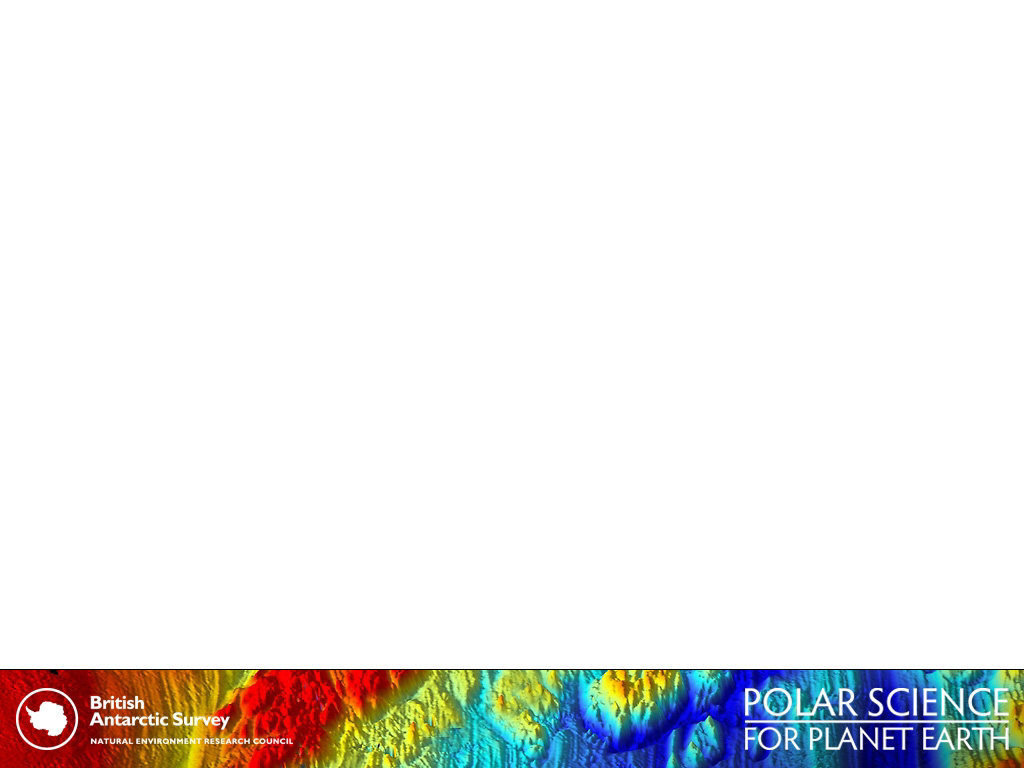
\includegraphics[width=720pt,height=540pt]{latexImage_0bbbcdc264c8ba747f2e5d9a88383de2.png}}
\put(48.45001,-60.06732){\fontsize{22}{1}\usefont{T1}{ptm}{b}{n}\selectfont\color{color_29791}Developer Environment}
\put(48.20001,-116.0331){\fontsize{16.5}{1}\usefont{T1}{ptm}{m}{n}\selectfont\color{color_29791}•}
\put(62.20001,-116.0331){\fontsize{16}{1}\usefont{T1}{ptm}{m}{n}\selectfont\color{color_29791}Use git!}
\put(48.20001,-150.2331){\fontsize{16.5}{1}\usefont{T1}{ptm}{m}{n}\selectfont\color{color_29791}•}
\put(62.20001,-150.2331){\fontsize{16}{1}\usefont{T1}{ptm}{m}{n}\selectfont\color{color_29791}Repeatable, reproducible \& shareable - containers can help}
\end{picture}
\newpage
\begin{tikzpicture}[overlay]\path(0pt,0pt);\end{tikzpicture}
\begin{picture}(-5,0)(2.5,0)
\put(-15,-530){
\includegraphics[width=720pt,height=540pt]{latexImage_ce4d9623382f08f383dd59532cc43efc.png}}
\put(48.45001,-60.06732){\fontsize{22}{1}\usefont{T1}{ptm}{b}{n}\selectfont\color{color_29791}Best Practice}
\put(48.20001,-116.0331){\fontsize{16.5}{1}\usefont{T1}{ptm}{m}{n}\selectfont\color{color_29791}•}
\put(62.20001,-116.0331){\fontsize{16}{1}\usefont{T1}{ptm}{m}{n}\selectfont\color{color_29791}User Policy}
\put(84.20001,-145.3436){\fontsize{12.5}{1}\usefont{T1}{ptm}{m}{n}\selectfont\color{color_29791}•}
\put(98.20001,-145.3436){\fontsize{12}{1}\usefont{T1}{ptm}{m}{n}\selectfont\color{color_29791}Link: }
\put(48.20001,-178.6331){\fontsize{16.5}{1}\usefont{T1}{ptm}{m}{n}\selectfont\color{color_29791}•}
\put(62.20001,-178.6331){\fontsize{16}{1}\usefont{T1}{ptm}{m}{n}\selectfont\color{color_29791}Do!}
\put(84.20001,-207.9436){\fontsize{12.5}{1}\usefont{T1}{ptm}{m}{n}\selectfont\color{color_29791}•}
\put(98.20001,-207.9436){\fontsize{12}{1}\usefont{T1}{ptm}{m}{n}\selectfont\color{color_29791}Ask for help, }
\put(48.20001,-269.6331){\fontsize{16.5}{1}\usefont{T1}{ptm}{m}{n}\selectfont\color{color_29791}•}
\put(62.20001,-269.6331){\fontsize{16}{1}\usefont{T1}{ptm}{m}{n}\selectfont\color{color_29791}Don't!}
\put(84.20001,-298.9436){\fontsize{12.5}{1}\usefont{T1}{ptm}{m}{n}\selectfont\color{color_29791}•}
\put(98.20001,-298.9436){\fontsize{12}{1}\usefont{T1}{ptm}{m}{n}\selectfont\color{color_29791}Submit jobs which use more than 4 nodes at a time.}
\end{picture}
\newpage
\begin{tikzpicture}[overlay]\path(0pt,0pt);\end{tikzpicture}
\begin{picture}(-5,0)(2.5,0)
\put(-15,-530){
\includegraphics[width=720pt,height=540pt]{latexImage_ffb5cd55fca49886e243ec0781935996.png}}
\put(48.45001,-60.06732){\fontsize{22}{1}\usefont{T1}{ptm}{b}{n}\selectfont\color{color_29791}HELP!}
\put(48.20001,-116.0331){\fontsize{16.5}{1}\usefont{T1}{ptm}{m}{n}\selectfont\color{color_29791}•}
\put(62.20001,-116.0331){\fontsize{16}{1}\usefont{T1}{ptm}{m}{n}\selectfont\color{color_29791}Service desk: }
\put(162.7,-116.0331){\fontsize{16}{1}\usefont{T1}{ptm}{m}{n}\selectfont\color{color_232414}servicedesk@bas.ac.uk}
\end{picture}
\begin{tikzpicture}[overlay]
\path(0pt,0pt);
\filldraw[color_232414][even odd rule]
(162.7pt, -117.6331pt) -- (331.825pt, -117.6331pt)
;
\end{tikzpicture}
\begin{picture}(-5,0)(2.5,0)
\put(48.20001,-150.2331){\fontsize{16.5}{1}\usefont{T1}{ptm}{m}{n}\selectfont\color{color_29791}•}
\put(62.20001,-150.2331){\fontsize{16}{1}\usefont{T1}{ptm}{m}{n}\selectfont\color{color_29791}HPC User Guide: }
\put(190.2,-150.2331){\fontsize{16}{1}\usefont{T1}{ptm}{m}{n}\selectfont\color{color_232414}http://ictdocs/wiki/index.php?title=HPC:User\_Guide}
\end{picture}
\begin{tikzpicture}[overlay]
\path(0pt,0pt);
\filldraw[color_232414][even odd rule]
(190.2pt, -151.8331pt) -- (551.45pt, -151.8331pt)
;
\end{tikzpicture}
\begin{picture}(-5,0)(2.5,0)
\put(48.20001,-218.6331){\fontsize{16.5}{1}\usefont{T1}{ptm}{m}{n}\selectfont\color{color_29791}•}
\put(62.20001,-218.6331){\fontsize{16}{1}\usefont{T1}{ptm}{m}{n}\selectfont\color{color_29791}Service Desk Solutions}
\put(48.20001,-252.8331){\fontsize{16.5}{1}\usefont{T1}{ptm}{m}{n}\selectfont\color{color_29791}•}
\put(62.20001,-252.8331){\fontsize{16}{1}\usefont{T1}{ptm}{m}{n}\selectfont\color{color_29791}Y}
\put(71.68801,-252.8331){\fontsize{16}{1}\usefont{T1}{ptm}{m}{n}\selectfont\color{color_29791}ammer}
\put(48.20001,-287.0331){\fontsize{16.5}{1}\usefont{T1}{ptm}{m}{n}\selectfont\color{color_29791}•}
\put(62.20001,-287.0331){\fontsize{16}{1}\usefont{T1}{ptm}{m}{n}\selectfont\color{color_29791}Email List}
\end{picture}
\newpage
\begin{tikzpicture}[overlay]\path(0pt,0pt);\end{tikzpicture}
\begin{picture}(-5,0)(2.5,0)
\put(-15,-530){
\includegraphics[width=720pt,height=540pt]{latexImage_432c55c52c2b004ff7b76272af817a3a.png}}
\put(243.25,-207.0516){\fontsize{28}{1}\usefont{T1}{ptm}{m}{n}\selectfont\color{color_29791}Any Questions? }
\end{picture}
\newpage
\begin{tikzpicture}[overlay]
\path(0pt,0pt);
\filldraw[color_283006][even odd rule]
(-15pt, 10pt) -- (705pt, 10pt)
 -- (705pt, 10pt)
 -- (705pt, -530pt)
 -- (705pt, -530pt)
 -- (-15pt, -530pt) -- cycle
;
\end{tikzpicture}
\begin{picture}(-5,0)(2.5,0)
\put(113.7764,-46.60965){\fontsize{44}{1}\usefont{T1}{ptm}{m}{n}\selectfont\color{color_29791}The Following }
\put(397.4444,-46.60965){\fontsize{44}{1}\usefont{T1}{ptm}{m}{n}\selectfont\color{color_29791}Are Slide }
\put(244.6885,-99.40967){\fontsize{44}{1}\usefont{T1}{ptm}{m}{n}\selectfont\color{color_29791}T}
\put(266.7325,-99.40967){\fontsize{44}{1}\usefont{T1}{ptm}{m}{n}\selectfont\color{color_29791}emplates}
\end{picture}
\newpage
\begin{tikzpicture}[overlay]\path(0pt,0pt);\end{tikzpicture}
\begin{picture}(-5,0)(2.5,0)
\put(-15,-530){
\includegraphics[width=720pt,height=540pt]{latexImage_432c55c52c2b004ff7b76272af817a3a.png}}
\put(48.45001,-207.0516){\fontsize{28}{1}\usefont{T1}{ptm}{m}{n}\selectfont\color{color_29791}T}
\put(64.52201,-207.0516){\fontsize{28}{1}\usefont{T1}{ptm}{m}{n}\selectfont\color{color_29791}itle}
\end{picture}
\newpage
\begin{tikzpicture}[overlay]\path(0pt,0pt);\end{tikzpicture}
\begin{picture}(-5,0)(2.5,0)
\put(-15,-530){
\includegraphics[width=720pt,height=540pt]{latexImage_8e9c8e6734598745b849b301599f41ac.png}}
\put(48.45001,-60.06732){\fontsize{22}{1}\usefont{T1}{ptm}{b}{n}\selectfont\color{color_29791}T}
\put(61.49601,-60.06732){\fontsize{22}{1}\usefont{T1}{ptm}{b}{n}\selectfont\color{color_29791}itle}
\end{picture}
\newpage
\begin{tikzpicture}[overlay]\path(0pt,0pt);\end{tikzpicture}
\begin{picture}(-5,0)(2.5,0)
\put(-15,-530){
\includegraphics[width=720pt,height=540pt]{latexImage_ffb5cd55fca49886e243ec0781935996.png}}
\put(48.45001,-60.06732){\fontsize{22}{1}\usefont{T1}{ptm}{b}{n}\selectfont\color{color_29791}T}
\put(61.49601,-60.06732){\fontsize{22}{1}\usefont{T1}{ptm}{b}{n}\selectfont\color{color_29791}itle}
\end{picture}
\newpage
\begin{tikzpicture}[overlay]\path(0pt,0pt);\end{tikzpicture}
\begin{picture}(-5,0)(2.5,0)
\put(-15,-530){
\includegraphics[width=720pt,height=540pt]{latexImage_c150d6a5d31e56fa54dc2f27c6d29c24.png}}
\put(48.45001,-60.06732){\fontsize{22}{1}\usefont{T1}{ptm}{b}{n}\selectfont\color{color_29791}T}
\put(61.49601,-60.06732){\fontsize{22}{1}\usefont{T1}{ptm}{b}{n}\selectfont\color{color_29791}itle}
\end{picture}
\newpage
\begin{tikzpicture}[overlay]\path(0pt,0pt);\end{tikzpicture}
\begin{picture}(-5,0)(2.5,0)
\put(-15,-530){
\includegraphics[width=720pt,height=540pt]{latexImage_0576cd716feb43c0bdb900476e5c8735.png}}
\put(48.45001,-60.06732){\fontsize{22}{1}\usefont{T1}{ptm}{b}{n}\selectfont\color{color_29791}T}
\put(61.49601,-60.06732){\fontsize{22}{1}\usefont{T1}{ptm}{b}{n}\selectfont\color{color_29791}itle}
\end{picture}
\newpage
\begin{tikzpicture}[overlay]\path(0pt,0pt);\end{tikzpicture}
\begin{picture}(-5,0)(2.5,0)
\put(-15,-530){
\includegraphics[width=720pt,height=540pt]{latexImage_0c7e336018b624b6d33eacc011f59acd.png}}
\put(48.45001,-60.06732){\fontsize{22}{1}\usefont{T1}{ptm}{b}{n}\selectfont\color{color_29791}T}
\put(61.49601,-60.06732){\fontsize{22}{1}\usefont{T1}{ptm}{b}{n}\selectfont\color{color_29791}itle}
\end{picture}
\newpage
\begin{tikzpicture}[overlay]\path(0pt,0pt);\end{tikzpicture}
\begin{picture}(-5,0)(2.5,0)
\put(-15,-530){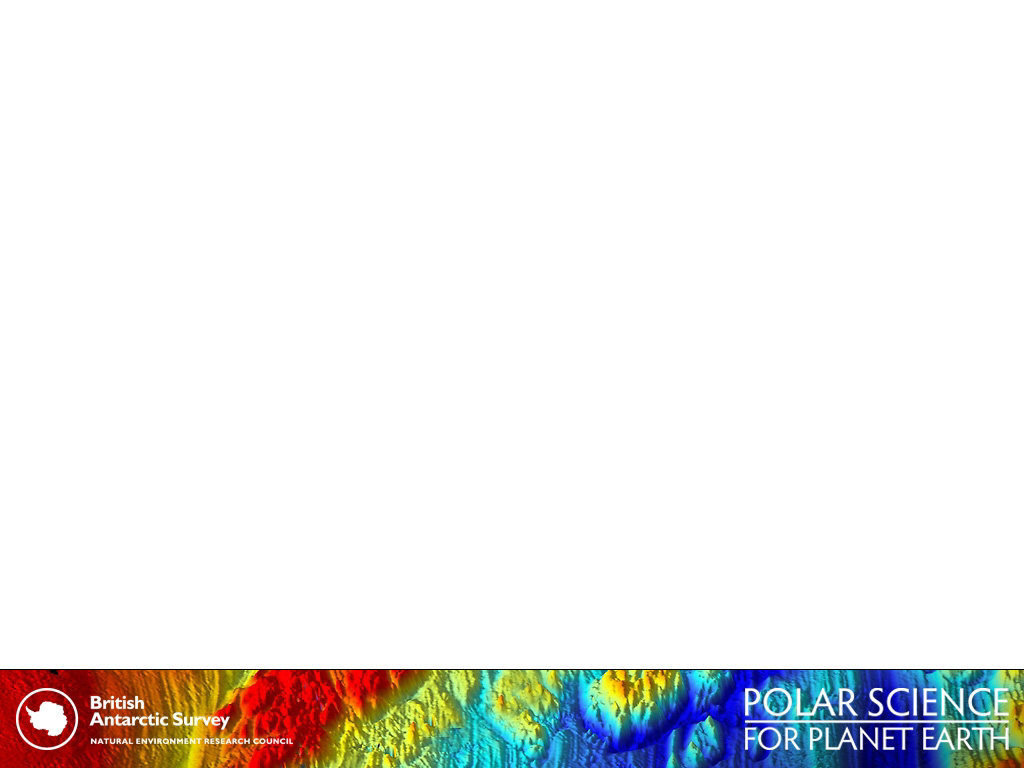
\includegraphics[width=720pt,height=540pt]{latexImage_0bbbcdc264c8ba747f2e5d9a88383de2.png}}
\put(48.45001,-60.06732){\fontsize{22}{1}\usefont{T1}{ptm}{b}{n}\selectfont\color{color_29791}T}
\put(61.49601,-60.06732){\fontsize{22}{1}\usefont{T1}{ptm}{b}{n}\selectfont\color{color_29791}itle}
\end{picture}
\newpage
\begin{tikzpicture}[overlay]\path(0pt,0pt);\end{tikzpicture}
\begin{picture}(-5,0)(2.5,0)
\put(-15,-530){
\includegraphics[width=720pt,height=540pt]{latexImage_74554d3b0f5b45b9b07769003a1a7e32.png}}
\put(48.45001,-60.06732){\fontsize{22}{1}\usefont{T1}{ptm}{b}{n}\selectfont\color{color_29791}T}
\put(61.49601,-60.06732){\fontsize{22}{1}\usefont{T1}{ptm}{b}{n}\selectfont\color{color_29791}itle}
\end{picture}
\newpage
\begin{tikzpicture}[overlay]\path(0pt,0pt);\end{tikzpicture}
\begin{picture}(-5,0)(2.5,0)
\put(-15,-530){
\includegraphics[width=720pt,height=540pt]{latexImage_7069de0bfaaa04bee2183ad80a89032d.png}}
\put(48.45001,-60.06732){\fontsize{22}{1}\usefont{T1}{ptm}{b}{n}\selectfont\color{color_29791}T}
\put(61.49601,-60.06732){\fontsize{22}{1}\usefont{T1}{ptm}{b}{n}\selectfont\color{color_29791}itle}
\end{picture}
\newpage
\begin{tikzpicture}[overlay]\path(0pt,0pt);\end{tikzpicture}
\begin{picture}(-5,0)(2.5,0)
\put(-15,-530){
\includegraphics[width=720pt,height=540pt]{latexImage_ce4d9623382f08f383dd59532cc43efc.png}}
\put(48.45001,-60.06732){\fontsize{22}{1}\usefont{T1}{ptm}{b}{n}\selectfont\color{color_29791}T}
\put(61.49601,-60.06732){\fontsize{22}{1}\usefont{T1}{ptm}{b}{n}\selectfont\color{color_29791}itle}
\end{picture}
\end{document}